\begin{table}
\caption{Notations and symbols used in this paper}\label{tab1}
\begin{center}
\begin{tabular}{|@{}l|c@{}|@{}l|c@{}|}
\hline
Symbols & Description & Symbols & Description\\
\hline
$[n]$ & $\{1, 2, \ldots, n\}$ & $\Pbf$ & Edge connectivity probability matrix\\
$\mathcal{G}$ & Graph & $\B$ & Block connectivity probability matrix\\
$n$ & Number of nodes & $\vec{\tau}$ & Vertex community assignment vector\\
$\A$ & Adjacency matrix & $\M$ & Edge community assignment matrix\\
$\A_i$ & $i$-th row of $\A$ & $\X$ & Latent position matrix\\
$\A_{ij}$ & $(i,j)$ entry of $\A$ & $\hat{\X}$ & Estimated latent position matrix\\
$\A^{(l)}$ & $l$-th element in sequence of $\A$ & &\\
\hline
\end{tabular}
\end{center}
\end{table}

\section{Statistical Models}\label{sec:models}
Connectomes can be modelled using statistical models designed for network data \cite{ goldenberg2010survey, kolaczyk2014statistical}. Statistical models consider the entire network as a random variable, including the inherent structure, dependencies within networks, and the noise in observed data. 
Thus, statistical models can formalize detecting similarities or differences for each of the representations in Section \ref{sec:representations}.
This section provides an overview of many statistical models for network data, including those designed for representing single and multiple networks. 

Section \ref{sec:single_graph_models} provides an overview of single graph models that have been extensively studied as well as recently introduced models in the order of least to greatest complexity. Figure \ref{fig:models}a shows the relationship between all the single graph models presented in this paper. Section \ref{sec:multi_graph_models} provides an overview of some models for multiple networks. While other statistical models for multiple network data exist \cite{zhang2018network, wang2019joint, nielsen2018multiple, Durante2017-fz}, we focus on  some recent models that are used in spectral inference for connectomics data. In Appendix \ref{sec:model_extensions}, we describe some extensions to these models. 

\begin{figure}
    \centering
    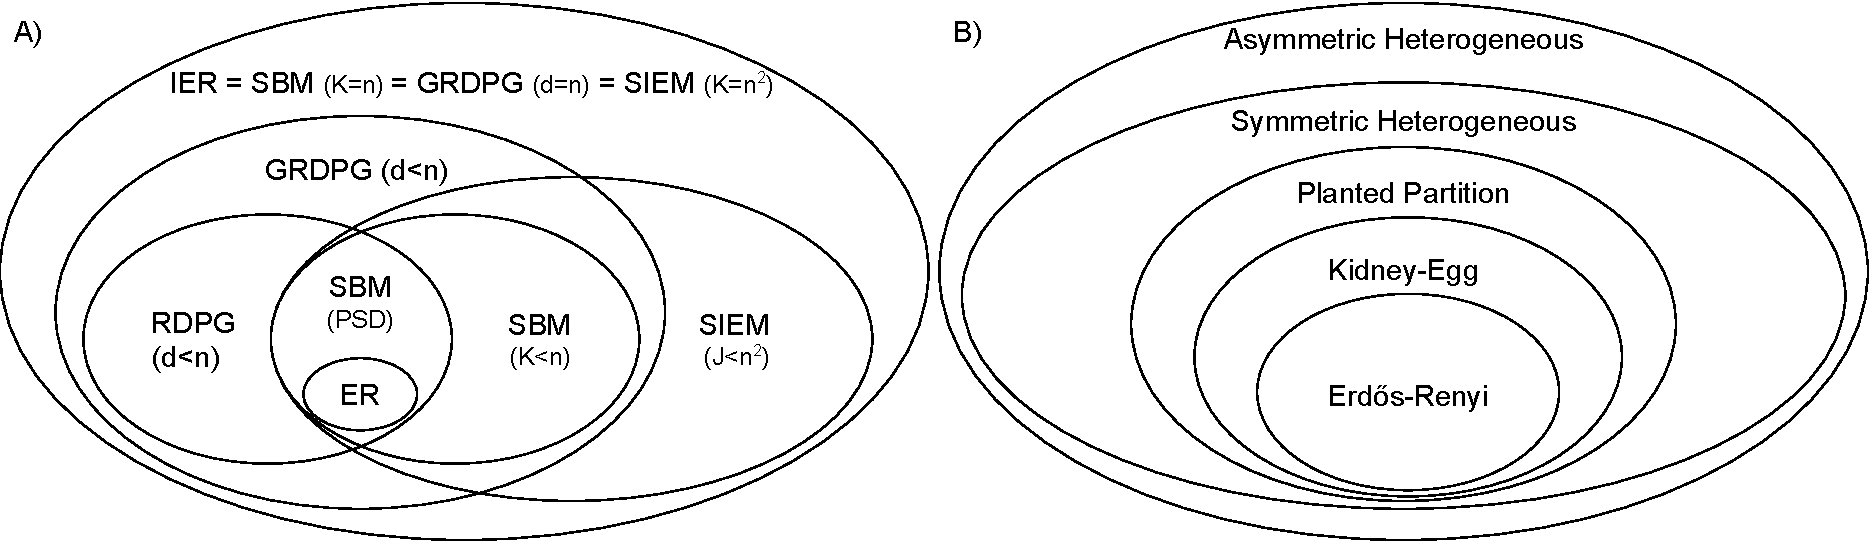
\includegraphics[width=\textwidth]{figures/dnd/models_combined}
    \caption
    [Hierarchical Relationships of Statistical Models]
    {\textbf{Hierarchical Relationships of Statistical Models} 
    \textbf{(a)} Relationships among all the single-graph statistical models. Erd\H os-R\'enyi ($\er$) model is a stochastic block model ($\sbm$) with one community. $\sbm$ with a positive semidefinite block probability matrix $\B$ is also a random dot product graph ($\rdpg$). Any $\sbm$, $\rdpg$, and some structured independent edge model ($\siem$) can be represented as $d$-dimensional generalized random dot product graph ($\grdpg$) with $d$ less than number of vertices $n$. Inhomogenous Erd\H os-R\'enyi ($\ier$) model is equivalent to a $n$-block $\sbm$, $n$-dimensional $\grdpg$, and $n^2$-group $\siem$.
    \textbf{(b)} Relationships among the two-block $\sbm$ models. The most complex model is the asymmetric heterogeneous $\sbm$, and the simplest model is the $\er$, which is a degenerate case of 2-block $\sbm$.}
    \label{fig:models}
\end{figure}

\subsection{Single Graph Models}\label{sec:single_graph_models}
\subsubsection{Erd\H os-R\'enyi Random Graphs (ER)}\label{sec:uer}
The simplest random graph model is the $\mathsf{Erd\ddot{o}s-R\acute{e}nyi~(ER)}$ model \cite{Erdos1959-zf}. For a given set of $n$ vertices, each distinct pair of vertices are connected independently with probability $p \in [0, 1]$. Specifically, $\A \sim\er_n(p)$ if $\A$ has entries $\A_{ij}\sim\bern(p)$ for $i, j \in [n]$. While the $\er$ model is not representative of real data, it has been studied extensively since many of its properties can be solved exactly  \cite{newman2003random,Rukhin2010}.  

\subsubsection{Stochastic Block Model (SBM)}\label{sec:usbm}
First introduced in \cite{holland1983stochastic}, $\sbm$ is a model that can produce graphs with vertices grouped into $K$ communities \cite{Rohe2011-ha,sussman2012consistent,Wasserman1987-tw}. There are two simple variations of the $\sbm$ in which the vertex assignment vector $\vec \tau \in \left\{1, \hdots, K\right\}^n$ is known \textit{a priori}, and where $\vec \tau$ is not known. 
In both cases, a symmetric $K \times K$ block connectivity probability matrix $\B$ with entries in $[0,1]^{K \times K}$ governs the probability of an edge between vertices given their block memberships. 

If $\vec \tau \in \left\{1, \hdots, K\right\}^n$ is known \textit{a priori}, the \textit{a priori} $\sbm$ is parametrized only by the block connectivity matrix $\B$, and the model is $\A \sim \sbm_n(\vec \tau,\B)$ if $\A$ has entries $\A_{ij} \sim \bern(\B_{kl})$ where $\tau_i = k, \tau_j = l$, for $i, j \in [n]$, and $k, l \in [K]$. In the case where $\vec \tau$ is not known, the \textit{a posteriori} $\sbm$ is additionally parameterized by a block membership probability vector $\vec{\pi} = [\pi_1,\dots,\pi_K]^\top$ on the probability simplex.
The model is $\A \sim \sbm_n(\vec \pi,\B)$ if $\A$ has entries $\A_{ij} \big | k=\tau_i, l=\tau_j \sim \bern(\B_{kl})$, where $\tau_i {\sim} \multinomial(\vec \pi)$ for $i = 1, \hdots, n$. 

Throughout the context of this paper, we will focus particularly on a few variations of the two-block $\sbm$ ($K=2$) with block connectivity matrix $\B = \begin{bmatrix}a & b \\ c & d \end{bmatrix}$, abbreviated as $\B = [a, b; c, d]$. The common variants include:
\begin{enumerate}
    \item $\mathsf{Kidney-Egg}$: $b = c = d$. In this model, one of the blocks has edges with a different probability than the others, but the remaining blocks are homogeneous, where $a \neq b$. Furthermore, when $b > a$, the model is referred to as core-periphery $\sbm$.
    \item $\mathsf{Planted~Partition}$: $a = d$ and $b = c$. In this model, the within-block edges share a common probability $a$, and the between-block edges share a common probability $b$, where $a \neq b$.
    \item $\mathsf{Symmetric~ Heterogeneous}$: $b = c$. In this model, the between-block edges share a common probability $b$, but the within-block edges have a disparate probabilities, where $a \neq b \neq d$. 
    \item $\mathsf{Asymmetric~ Heterogeneous}$: $a \neq b \neq c \neq d$. In this directed model, every block has a unique probability.
    \item $\mathsf{Erd\ddot{o}s-R\acute{e}nyi}$: $a=b=c=d$. In this degenerate model, all blocks have a common probability, and the partitioning is irrelevant. 
    \item $\mathsf{Homophilic/Assortative/Affinity}$: $a, d > b, c$. In this model, the within-block probabilities are greater than cross-block probabilities.
    \item $\mathsf{Disassortative}$: $ b, c > a, d$. In this model, the cross-block probabilities are greater than the within-block probabilities.
\end{enumerate}
Figure \ref{fig:models}b summarizes the relationships of $\sbm$ models.

\subsubsection{Structured Independent Edge Model (SIEM)}\label{sec:usiem}
$\siem$ is a generalization of $\sbm$ that produces graphs in which edges are grouped into one of $K$ clusters. Analogous to the vertex assignment vector of the \textit{a priori} $\sbm$, the $\siem$ features an edge community assignment matrix $\M \in \left\{1, \hdots, K\right\}^{n \times n}$ which is known \textit{a priori}. Given the community assignment matrix $\M$, the $\siem$ is $\A \sim \siem_n(\M, \vec p)$ if $\A_{ij} {\sim}\bern(p_k)$ where $\M_{ij} = k$, for $i, j \in [n]$ and $k \in [K]$. $\vec p = [p_1, \hdots, p_K]^\top \in [0, 1]^K$ is the edge probability vector which governs the probability of an edge between vertices. 

The \textit{a priori} $\sbm$ is a special case of $\siem$ in which edges are assigned to blocks $\M$ which respect the vertex assignment vector $\vec \tau$. For the purposes of this paper, we will consider a case that frequently comes up in neuroimaging, the $\mathsf{Homotopic~ SIEM}$, in which each vertex has a matched ``pair'' amongst other vertices. The edges corresponding to a pair $\M_{ij} = 2$ where $(v_i, v_j)$ are a pair of vertices sharing a property, and the edges corresponding to a non-pair are $\M_{ij} = 1$. A matched pair of vertices, for instance, could be homotopic brain regions (two brain regions with similar function but in opposing hemispheres of the brain).

\subsubsection{Random Dot Product Graphs (RDPG)}\label{sec:rdpg}
$\rdpg$ belongs to the class of latent position random graphs \cite{hoff2002latent}. In a latent position graph, every vertex has associated to it a (typically unobserved) \textit{latent position} in some space $\mathcal{X}$, and the probability of connection between vertices $i$ and $j$ are given by a link function. In $\rdpg$, the space $\mathcal{X}$ is a constrained subspace of Euclidean space $\RR^d$ and the link function is the dot product \cite{Young2007-vu,scheinerman2010modeling,Sussman2014-zq}. Thus, in a $d-$dimensional $\rdpg$ with $n$ vertices, the matrix $\X\in \RR^{n\times d}$ whose rows are the latent positions, and the matrix of connection probabilities is given by $\Pbf=\X\X^\top$, which is positive semidefinite. The model is $\A\sim \rdpg_n(\X)$ if the adjacency matrix $\A$ has entries $\A_{ij} \sim \bern(\X_i\X_j^\top)$.
Subsequent inference tasks include community detection \cite{sussman2012consistent}, vertex classification \cite{tang2013}, or two-sample hypothesis testing for graphs with matched and non-matched vertices for a pair of graphs  \cite{priebe2019two,tang2017nonparametric,tang2017semiparametric}.

The $\rdpg$ is a flexible model, and other models of interest can be seen as special cases of the $\rdpg$. A $\sbm$ whose block connectivity matrix $\B$ is positive semi-definite is a $\rdpg$ with $K$ distinct latent positions. Thus, a $\sbm$ with $K$ blocks can be represented with a latent position matrix $\X\in\RR^{n\times d}$, with $d\leq K$, where there are only $K$ different rows of $\X$, and letting $\X_{\mathcal{U}}\in\RR^{K\times d}$ be the matrix with the subset of the rows $\mathcal{U}$ where each row is the latent position for a block, then the block connectivity matrix is $\B= \X_\mathcal{U}\X_\mathcal{U}^\top \in\RR^{K\times K}$. More generally, the $\rdpg$ can represent other models with more complex structures, such as mixed memberships \cite{Airoldi2008-tp} or hierarchical communities \cite{Lyzinski2017-cq}.

\subsubsection{Generalized Random Dot Product Graphs (GRDPG)}\label{sec:grdpg}
Unlike $\rdpg$ model, $\grdpg$ does not assume that $\Pbf$ is a positive semidefinite probability matrix  \cite{rubin2017statistical}. In this model, the edge probability matrix is given by $\Pbf=\X \I_{pq}\X^\top$, and $\A\sim\grdpg_n(
\X, p, q)$ if $\A_{ij}\sim\bern(\X_i\I_{pq}\X_j^\top)$ where $\I_{pq}=\textrm{diag}(1, \ldots, 1, -1, \ldots, -1)$  with $p$ ones followed by $q$ minus ones on its diagonal, and where $p \geq 1$ and $q \geq 0$ are two integers satisfying $p + q = d$.

The $\grdpg$ generalizes all of the previous models. When $q=0$, $\grdpg$ reduces to a $\rdpg$ model. To represent any $\sbm$ as $\grdpg$, let $p\geq 1, q\geq 0$ be the number of positive and negative eigenvalues of the block connectivity matrix $\B\in\RR^{K\times K}$, respectively. The block matrix can be represented as $\B = \X_\mathcal{U}\I_{pq}\X_\mathcal{U}^\top$.

\subsubsection{Inhomogenous Erd\H os-R\'enyi Random Graphs (IER)}\label{sec:uierrg}
The $\mathsf{Inhomogenous~Erd\ddot{o}s-R\acute{e}nyi~(IER)}$ is a model where each pair of nodes has a unique probability of an edge existing between the two, and is therefore the most general independent edge model. For a given set of $n$ vertices, the $\ier$ is parametrized by a matrix $\Pbf \in [0, 1]^{n \times n}$, where $\Pbf_{ij}$ is the probability of an edge connecting vertices $v_i, v_j$ where $i, j \in [n]$. That is, $\A \sim \ier_n(\Pbf)$ if $\A$ has entries $\A_{ij}\sim \bern(\Pbf_{ij})$ for $i, j \in [n]$. $\ier$ cannot be estimated from a single graph, as there are $n\choose 2$ unknowns (the probabilities) with $n\choose 2$ total observations (the edges).

Note that all single graph models are special cases of $\ier$. Additionally, $\sbm$ with $K=n$, $\siem$ with $K=n^2$, and $\grdpg$ with $d=n$ are equivalent to an $\ier$ model.

\subsection{Multiple Graph Models}\label{sec:multi_graph_models}
A common idea in statistical models for multiple graphs is a shared latent space that contain structural information common to all graphs. The two models presented in this section constrain the shared latent space in different ways to describe the heterogeneity in graphs, which results in sensitivity to different kinds of heterogeneity. The advantages and disadvantages of each model are highlighted in Section \ref{sec:multi_app}.

In the following models, consider a sample of $m$ observed graphs $\mathcal{G}^{(1)}, \mathcal{G}^{(2)}, \ldots, \mathcal{G}^{(m)}$  and their associated adjacency matrices, $\A^{(1)}, \A^{(2)}, \ldots, \A^{(m)}\in\RR^{n\times n}$ with $n$ vertices that are identical and shared across all graphs. 

\subsubsection{Joint Random Dot Product Graphs (JRDPG)}
In this model, we consider a collection of $m$ $\rdpg$s all with the same generating latent positions. Similar to a $\rdpg$, given an appropriately constrained Euclidean subspace $\RR^d$, the model is parameterized by a latent positions matrix $\X\in\RR^{n\times d}$ where $d \ll n$. The model is $\left(\A^{(1)}, \A^{(2)}, \ldots, \A^{(m)}\right)\sim \jrdpg(\X)$ where $\A_{ij}^{(l)}\sim \bern(\X_i\X_j^\top)$ for all $i, j \in [n]$ and $l\in [m]$. Each graph has marginal distribution $\A^{(l)}\sim\rdpg(\X)$ for all $l \in [m]$, meaning that the matrices $\A^{(1)}, \ldots,\A^{(m)}$ are conditionally independent given $\X$ \cite{athreya2017statistical,levin2017central}. While the model assumes that the latent positions for the graphs are the same, we note that this assumption is likely violated in heterogeneous networks, but still remains a very useful model as shown in Section \ref{sec:multi_app}.

\subsubsection{Common Subspace Independent-Edge Model (COSIE)} \label{sec:cosie}
In this model, the heterogeneous networks are described via a shared latent structure on the vertices, but also permits sufficient heterogeneity via individual matrices for each graph  \cite{arroyo2019inference}.
The model is parameterized by a  matrix $\V\in\RR^{n\times d}$ with orthonormal columns, 
where $n$ is the number of vertices and $d\ll n$, and  symmetric individual score matrices $\R^{(i)}\in\RR^{d\times d}$. The matrix $\V$ characterizes a low-rank common subspace, and is related to the latent positions for the vertices, and the score matrices incorporate individual differences to model the heterogeneity of the graphs. The model is denoted by $\left(\A^{(1)}, \ldots, \A^{(m)}\right)\sim \cosie(\V; \R^{(1)}, \ldots, \R^{(m)})$ where $\A_{ij}^{(l)} \sim \bern(\mathbf{P}^{(l)}_{ij})$ for all $i, j\in [n], i < j$, and $\mathbf{P}^{(l)}=\V\R^{(l)}\V^\top$. This factorization of the expected adjacency matrices is related to other decompositions for multiple matrices into population singular vectors or eigenvectors and individual parameters \cite{afshin2012enhancing,crainiceanu2011population,lock2013joint,wang2019common}.

\subsubsection{Correlated Models} \label{sec:correlated-graphs}
Finally, we are interested in graph models for a pair of graphs, $\mathcal{G}_1$ and $\mathcal{G}_2$, where the two graphs are said to be correlated; that is, the edges adjoining incident vertices have a non-zero correlation. Correlated graph models have numerous applications, such as when a graph is estimated repeatedly for the same source at different points in time.

\paragraph{Correlated $(\Pbf,\Q)$}

The $\mathbf{R}$-correlated $(\Pbf, \Q)$ model \cite{lyzinski2017matchability} with parameters $\mathbf{R}, \Pbf, \Q\in[0,1]^{n\times n}$, denoted as $\mathrm{CorrER}(\Pbf, \Q, \mathbf{R})$, produces two graphs $\mathcal{G}_1$ and $\mathcal{G}_2$ with adjacency matrices $\A^{(1)}, \A^{(2)}$ such that each graph is marginally an inhomogeneous Erd\H{o}s-R\'enyi with $\A^{(1)} \sim \ier(\Pbf)$, $\A^{(2)}\sim \ier(\Q)$, but the  pairs of corresponding edges have Pearson correlation  encoded in the matrix $\mathbf{R}$ such that 
$$\mathbf{R}_{ij} = \text{Corr}(\A^{(1)}, \A^{(2)})= \frac{\mathbb{P}(\A^{(1)}_{ij}=\A^{(2)}_{ij}=1)-\Pbf_{ij}\Q_{ij}}{\sqrt{\Pbf_{ij}(1-\Pbf_{ij}) \Q_{ij}(1-\Q_{ij})}}.$$
When $\Pbf$ and $\Q$ are different, there are restrictions in the values that the correlation matrix $\mathbf{R}$ can take. In particular, if $\Pbf_{ij}\neq\Q_{ij}$  and $\Pbf>\Q$, then $\mathbf{R}_{ij}\leq \sqrt{\frac{\Q_{ij}(1-\Q_{ij})}{\Pbf_{ij}(1-\Pbf_{ij})}}$ \cite{lyzinski2017matchability}.

We are interested particularly in two special cases of the $\mathrm{CorrER}(\Pbf, \pmb Q, \pmb R)$:
\begin{enumerate}
    \item The $\rho$-correlated $\rdpg$ model arises when $\Pbf = \Q=\X\X^\top$ for some latent position matrix $\X \in \RR^{n \times d}$  as in Section \ref{sec:rdpg}, and $\pmb R = \rho \pmb 1_{n \times n}$ (that is, the matrix of edge correlations $\pmb R$ has only a single unique entry $\rho\geq 0$). We say that $\A_1, \A_2 \sim \rho\rdpg(\X)$.
    \item The $\rho$-correlated $\er$ model arises in the case where $\Pbf = \Q = p\pmb 1_{n \times n}$ (i.e.,  the probability matrix has a single unique entry $p>0$), and $\pmb R = \rho\pmb 1_{n \times n}$ (as above, the matrix of correlations has a single unique entry). We say that $\A_1, \A_2 \sim \rho\er(p)$.
\end{enumerate}